\clearpage
\section{Summary}
\label{sec:summary}
\subsection{Calculation of cross sections}
From the unfolding procedure described in the previous section, we obtain the unfolded $M_{3\pi}$ mass spectrum $\left( \frac{dN}{dm} \right)^{\text{unfold}}$ for each data-taking period. 
For practical analysis, we work in discrete mass bins. Let $\left( \frac{dN}{dm} \right)^{\text{unfold}}_i$ denote the unfolded yield in the $i$-th mass bin, and $\Delta L_i = \int_{m_i}^{m_{i+1}} \frac{dL}{dm} dm$ denote the integrated luminosity in that bin. The dressed cross section $\sigma_{3\pi}^{\text{dress}}(m)$ is then obtained by:
\begin{equation}
    \sigma_i^{\text{dress}} = \frac{\left( \frac{dN}{dm} \right)^{\text{unfold}}_i}{\Delta L_i \cdot \mathcal{B}(\pi^{0} \to \gamma\gamma)}
    \label{eq:dressed_cross_section}
\end{equation}
where $\mathcal{B}(\pi^{0} \to \gamma\gamma) = (98.823 \pm 0.034)\%$ is the branching fraction of $\pi^{0} \to \gamma\gamma$ as quoted by the Particle Data Group (PDG)~\cite{PDG2024}. The complete formula for calculating $\frac{dL}{dm}$ is provided in Sec.~\ref{sec:bkg_stu}.

The unfolding procedure yields not only the unfolded spectrum $\left( \frac{dN}{dm} \right)^{\text{unfold}}_i$ but also its covariance matrix $\mathbf{C}$, which fully describes the uncertainties and correlations of $\left( \frac{dN}{dm} \right)^{\text{unfold}}_i$. However, additional uncertainties arise from the luminosity measurement and the $\pi^0$ branching fraction. These must be propagated to the dressed cross section $\boldsymbol{\sigma}^{\text{dress}}$.

The integrated luminosity per bin $\Delta L_i$ is not a measured quantity but is calculated from the total integrated luminosity $L_{\text{total}}$ via $\Delta L_i = f_i \cdot L_{\text{total}}$, where $f_i = \frac{1}{L_{\text{total}}} \int_{m_i}^{m_{i+1}} \frac{d\mathcal{L}}{dm} dm$ is the theoretical shape factor determined from QED, considered to have negligible uncertainty. The total luminosity $L_{\text{total}}$ is measured with a relative uncertainty $\delta_L = \sigma_L / L_{\text{total}}$. For the present analysis, $\delta_L = 19.0 / 4995 \approx 0.38\%$. The luminosity uncertainty affects all mass bins in a {\it fully correlated} manner: if the measured total luminosity is overestimated by $1\%$, all $\Delta L_i$ are overestimated by $1\%$, and consequently all $\sigma_i^{\text{dress}}$ are underestimated by $1\%$. This full correlation is a crucial property of normalization uncertainties.

Similarly, the $\pi^0 \to \gamma\gamma$ branching fraction $\mathcal{B}$ is known from PDG with a relative uncertainty $\delta_{\mathcal{B}} = \sigma_{\mathcal{B}} / \mathcal{B} \approx 0.034\%$. This uncertainty is also {\it fully correlated} across all mass bins, since the same branching fraction is used to normalize every bin.

The total covariance matrix of the dressed cross section combines three independent sources of uncertainty: the statistical and systematic uncertainties from the unfolding (encoded in $\mathbf{C}$), the luminosity uncertainty, and the $\pi^0$ branching fraction uncertainty. These sources are independent, so their covariance matrices add linearly. The propagation proceeds as follows.

First, the unfolded spectrum covariance is propagated through division by $\Delta L_i \cdot \mathcal{B}$. With $\sigma_i^{\text{dress}} = \left( \frac{dN}{dm} \right)^{\text{unfold}}_i / (\Delta L_i \cdot \mathcal{B})$, the Jacobian matrix is diagonal with elements $\partial \sigma_i^{\text{dress}} / \partial \left( \frac{dN}{dm} \right)^{\text{unfold}}_j = \delta_{ij} / (\Delta L_i \cdot \mathcal{B})$. Therefore:
\begin{equation}
    \left[\mathbf{C}_{\sigma}^{\text{(unfold)}}\right]_{ij} = \frac{\left[\mathbf{C}\right]_{ij}}{(\Delta L_i \cdot \mathcal{B})(\Delta L_j \cdot \mathcal{B})} = \frac{\left[\mathbf{C}\right]_{ij}}{\Delta L_i \Delta L_j \mathcal{B}^2}
    \label{eq:unfold_covariance}
\end{equation}
or in matrix form $\mathbf{C}_{\sigma}^{\text{(unfold)}} = \mathbf{D} \cdot \mathbf{C} \cdot \mathbf{D}^T$, where $\mathbf{D} = \operatorname{diag}(1/(\Delta L_i \mathcal{B}))$.

Second, the luminosity uncertainty, being fully correlated, contributes a rank-1 covariance matrix:
\begin{equation}
    \left[\mathbf{C}_{\sigma}^{\text{(lumi)}}\right]_{ij} = \sigma_i^{\text{dress}} \cdot \sigma_j^{\text{dress}} \cdot \delta_L^2 = \delta_L^2 \cdot \boldsymbol{\sigma}^{\text{dress}} (\boldsymbol{\sigma}^{\text{dress}})^T
    \label{eq:lumi_covariance}
\end{equation}
The correlation coefficient between any two bins from this source is $\rho_{ij} = 1$, reflecting complete correlation.

Third, the $\pi^0$ branching fraction uncertainty, also fully correlated, contributes similarly:
\begin{equation}
    \left[\mathbf{C}_{\sigma}^{\text{(BR)}}\right]_{ij} = \sigma_i^{\text{dress}} \cdot \sigma_j^{\text{dress}} \cdot \delta_{\mathcal{B}}^2 = \delta_{\mathcal{B}}^2 \cdot \boldsymbol{\sigma}^{\text{dress}} (\boldsymbol{\sigma}^{\text{dress}})^T
    \label{eq:br_covariance}
\end{equation}

The total covariance matrix for the dressed cross section is then:
\begin{equation}
    \mathbf{C}_{\sigma}^{\text{(dress)}} = \mathbf{C}_{\sigma}^{\text{(unfold)}} + (\delta_L^2 + \delta_{\mathcal{B}}^2) \cdot \boldsymbol{\sigma}^{\text{dress}} (\boldsymbol{\sigma}^{\text{dress}})^T
    \label{eq:total_covariance}
\end{equation}

The total uncertainty for each bin is given by $\sigma_{\sigma_i^{\text{dress}}} = \sqrt{\left[\mathbf{C}_{\sigma}^{\text{(dress)}}\right]_{ii}}$. For a single bin, the relative uncertainty squares add quadratically:
\begin{equation}
    \left(\frac{\Delta \sigma_i^{\text{dress}}}{\sigma_i^{\text{dress}}}\right)^2 = \left(\frac{\Delta \left( \frac{dN}{dm} \right)^{\text{unfold}}_i}{\left( \frac{dN}{dm} \right)^{\text{unfold}}_i}\right)^2 + \delta_L^2 + \delta_{\mathcal{B}}^2
    \label{eq:relative_error_decomposition}
\end{equation}
where $\Delta \left( \frac{dN}{dm} \right)^{\text{unfold}}_i / \left( \frac{dN}{dm} \right)^{\text{unfold}}_i$ is the relative uncertainty from the unfolding. For the present analysis, $\delta_L \approx 0.38\%$ dominates over $\delta_{\mathcal{B}} \approx 0.034\%$, while the unfolding uncertainty varies with mass and is typically the largest contribution.

It is important to note that while the diagonal elements follow Eq.~\ref{eq:relative_error_decomposition}, the off-diagonal elements retain the correlation structures of each source. The luminosity and branching fraction uncertainties introduce 100\% correlations across all bins, while the unfolding covariance $\mathbf{C}$ contains the correlations determined by the unfolding procedure.

Using Eq.~\ref{eq:total_covariance}, we obtain four independent dressed cross section results $\sigma_{3\pi}^{\text{dress}}(m)$ corresponding to the four data-taking periods: Round~03/04, Round~15, Round~16, and Round~17. These results are presented in Fig.~\ref{fig:sigma_dress_results_all_rounds} along with their total uncertainties, which now properly include the luminosity and $\pi^0$ branching fraction contributions.

\begin{figure}[htbp]
    \centering

    % === Row 1: Round 03/04 ===
    \subfloat[Round 03/04, $\omega(782)$ region]{
        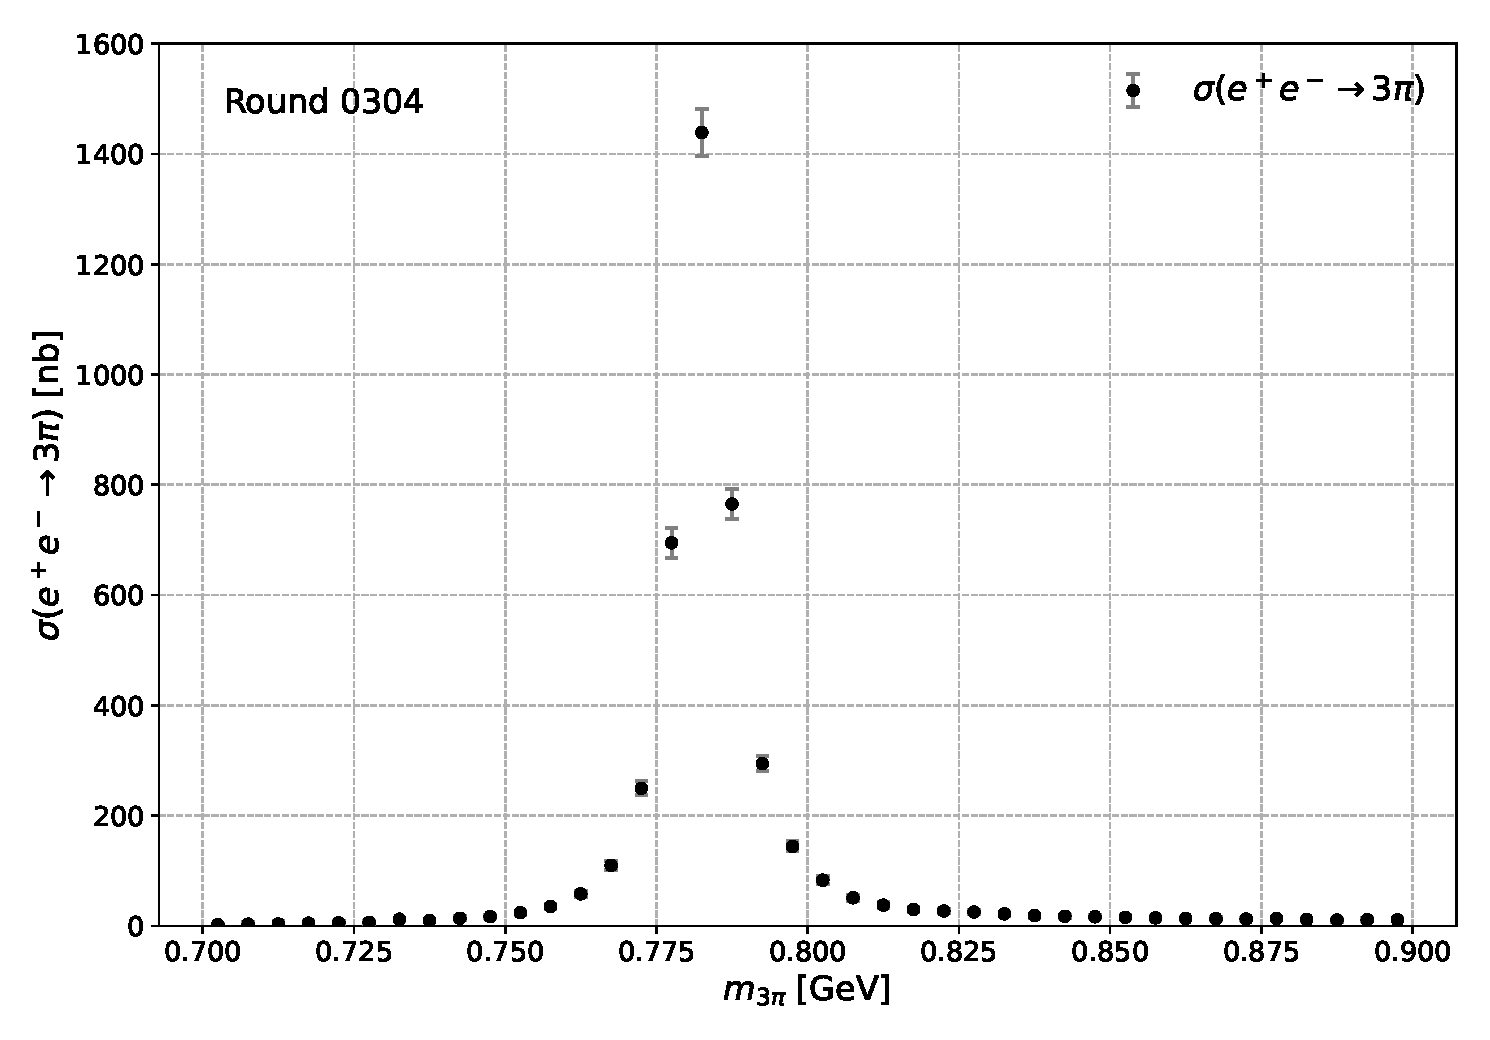
\includegraphics[width=0.32\textwidth]{fig/sigma_final_round0304_omega.eps}
        \label{fig:sigma_final_round0304_omega}
    }\hfill
    \subfloat[Round 03/04, $\phi(1020)$ region]{
        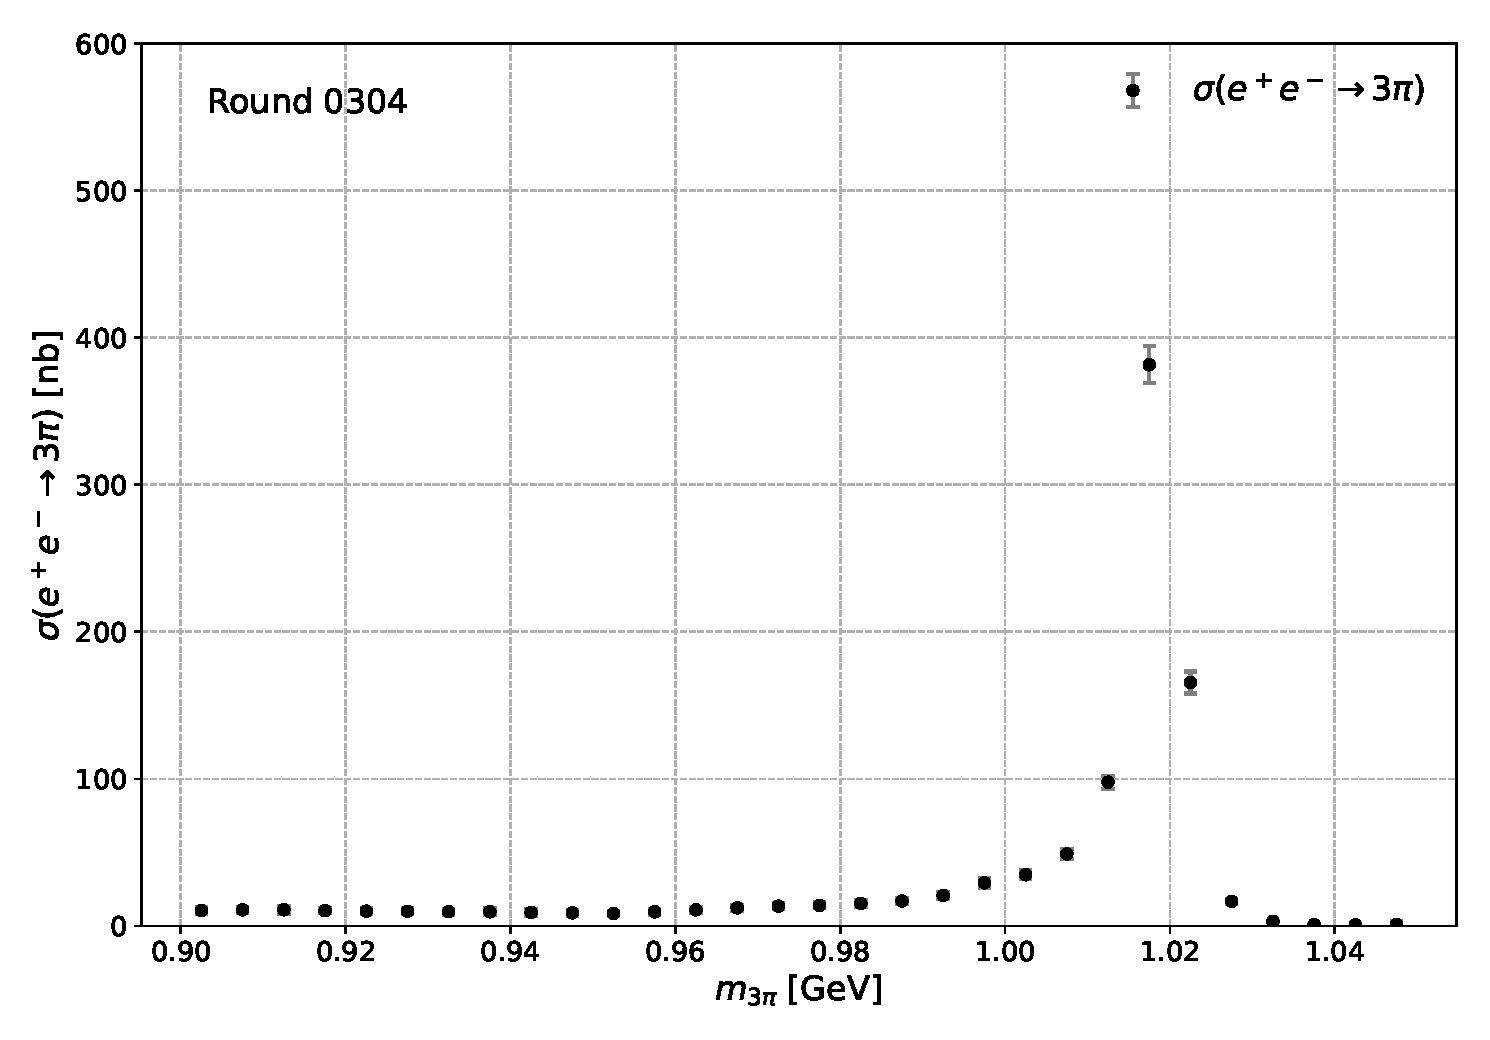
\includegraphics[width=0.32\textwidth]{fig/sigma_final_round0304_phi.eps}
        \label{fig:sigma_final_round0304_phi}
    }\hfill
    \subfloat[Round 03/04, $\omega^{\prime}/\omega^{\prime\prime}$ region]{
        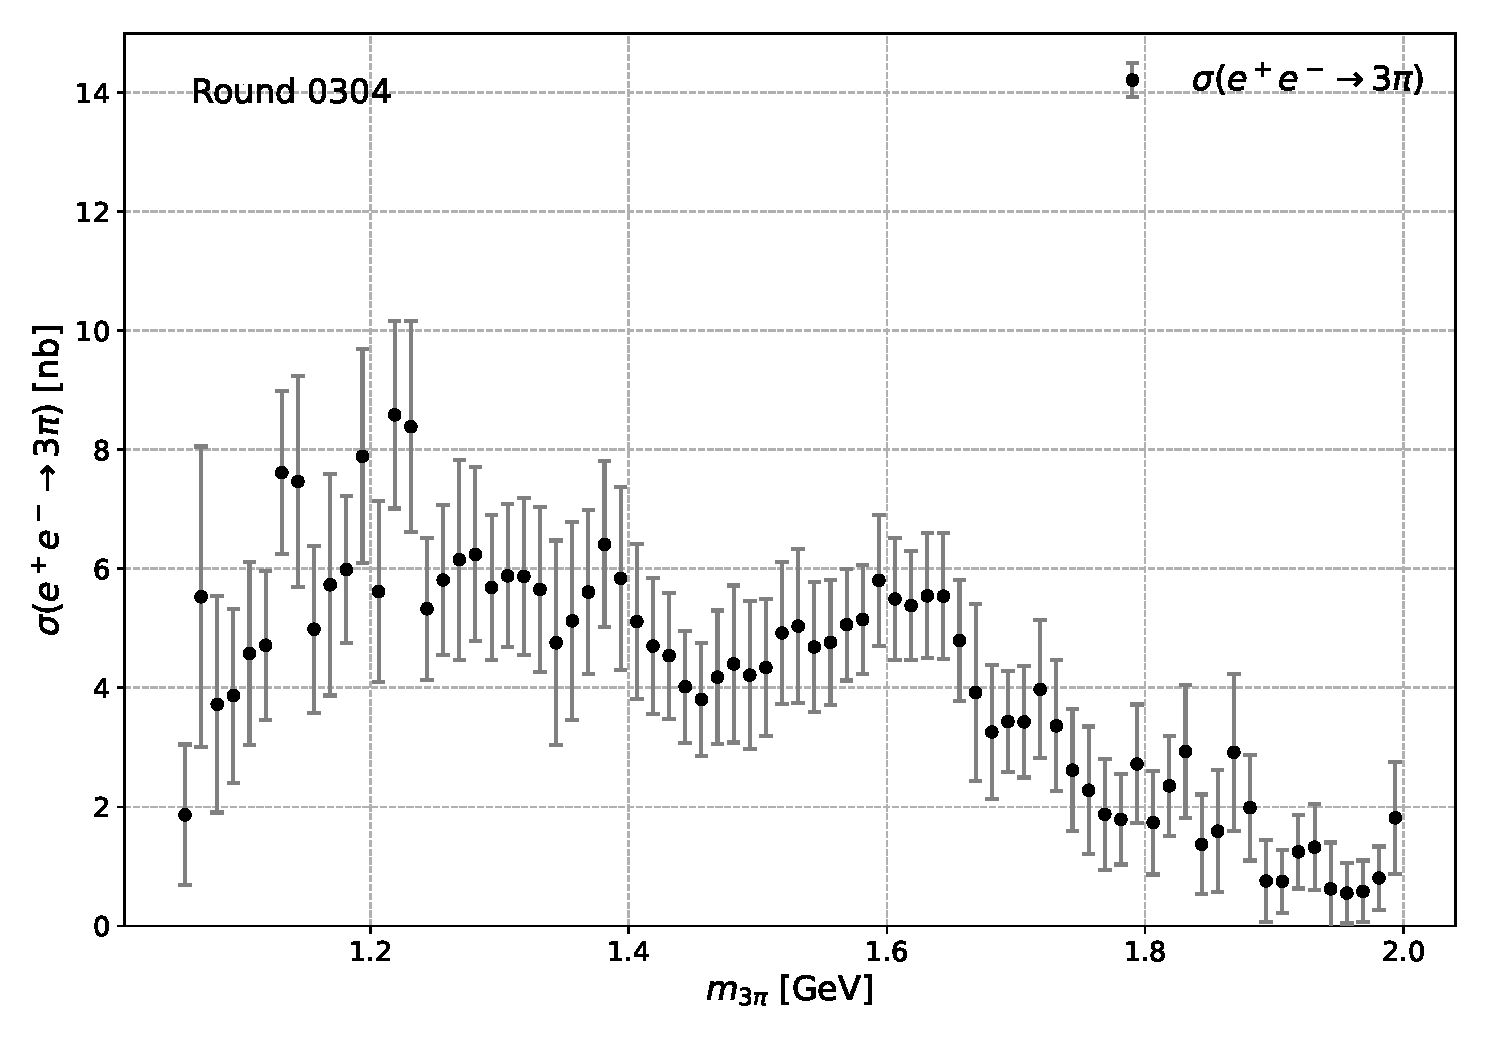
\includegraphics[width=0.32\textwidth]{fig/sigma_final_round0304_high.eps}
        \label{fig:sigma_final_round0304_high}
    }

    \vspace{0.5\baselineskip}

    % === Row 2: Round 15 ===
    \subfloat[Round 15, $\omega(782)$ region]{
        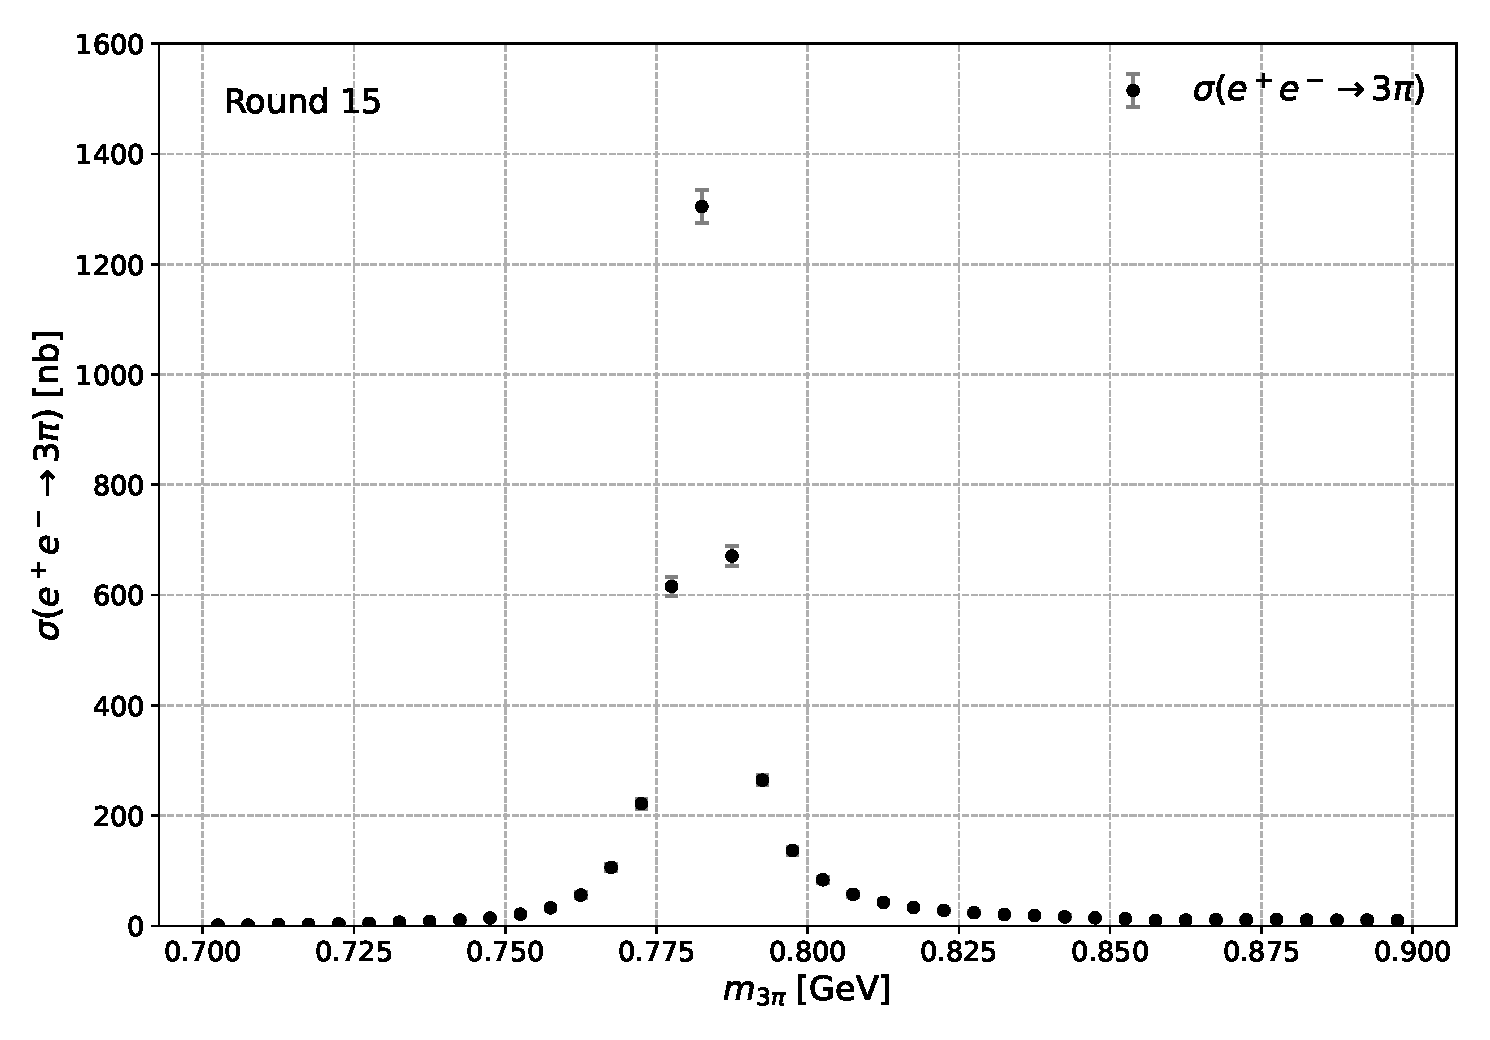
\includegraphics[width=0.32\textwidth]{fig/sigma_final_round15_omega.eps}
        \label{fig:sigma_final_round15_omega}
    }\hfill
    \subfloat[Round 15, $\phi(1020)$ region]{
        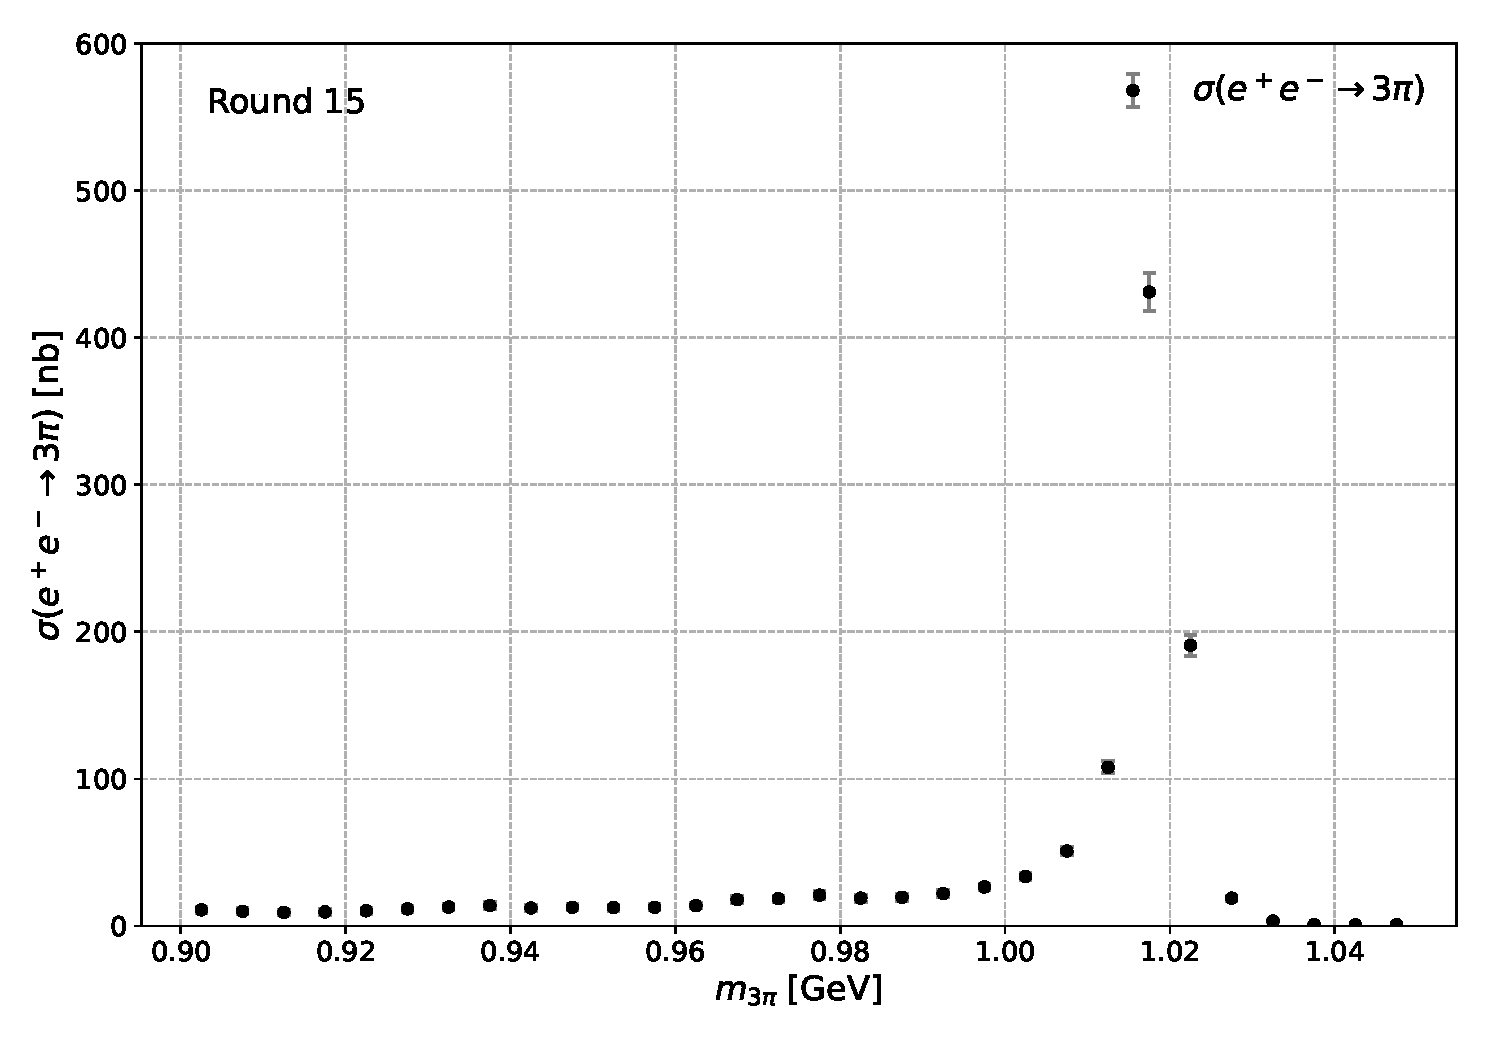
\includegraphics[width=0.32\textwidth]{fig/sigma_final_round15_phi.eps}
        \label{fig:sigma_final_round15_phi}
    }\hfill
    \subfloat[Round 15, $\omega^{\prime}/\omega^{\prime\prime}$ region]{
        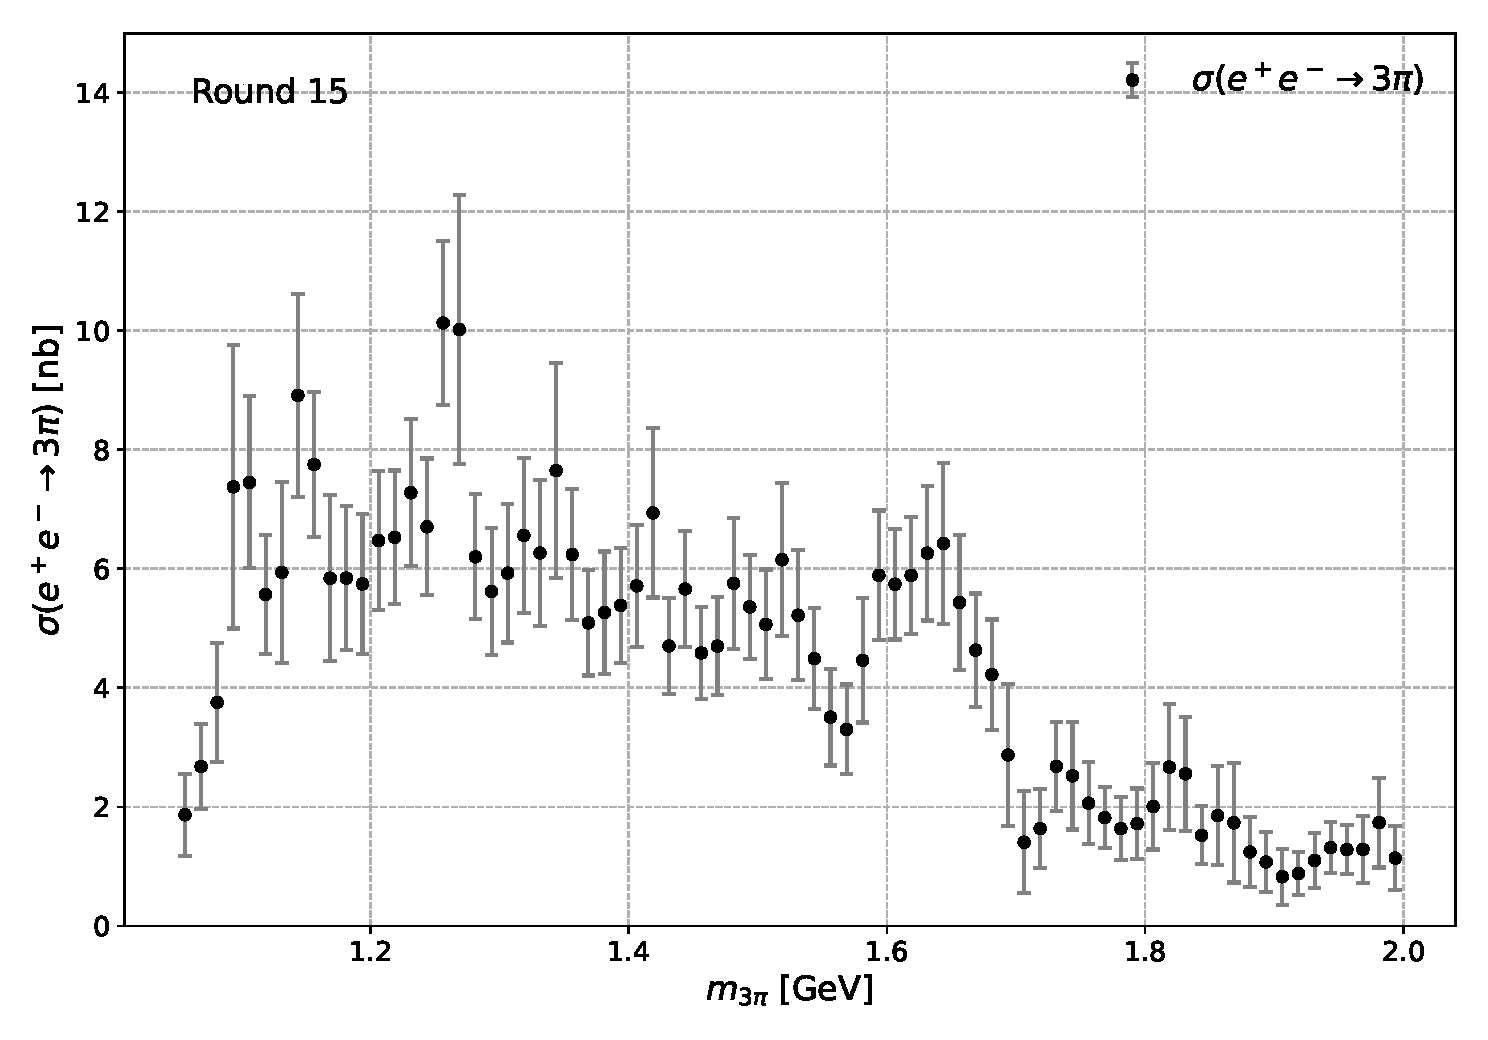
\includegraphics[width=0.32\textwidth]{fig/sigma_final_round15_high.eps}
        \label{fig:sigma_final_round15_high}
    }

    \vspace{0.5\baselineskip}

    % === Row 3: Round 16 ===
    \subfloat[Round 16, $\omega(782)$ region]{
        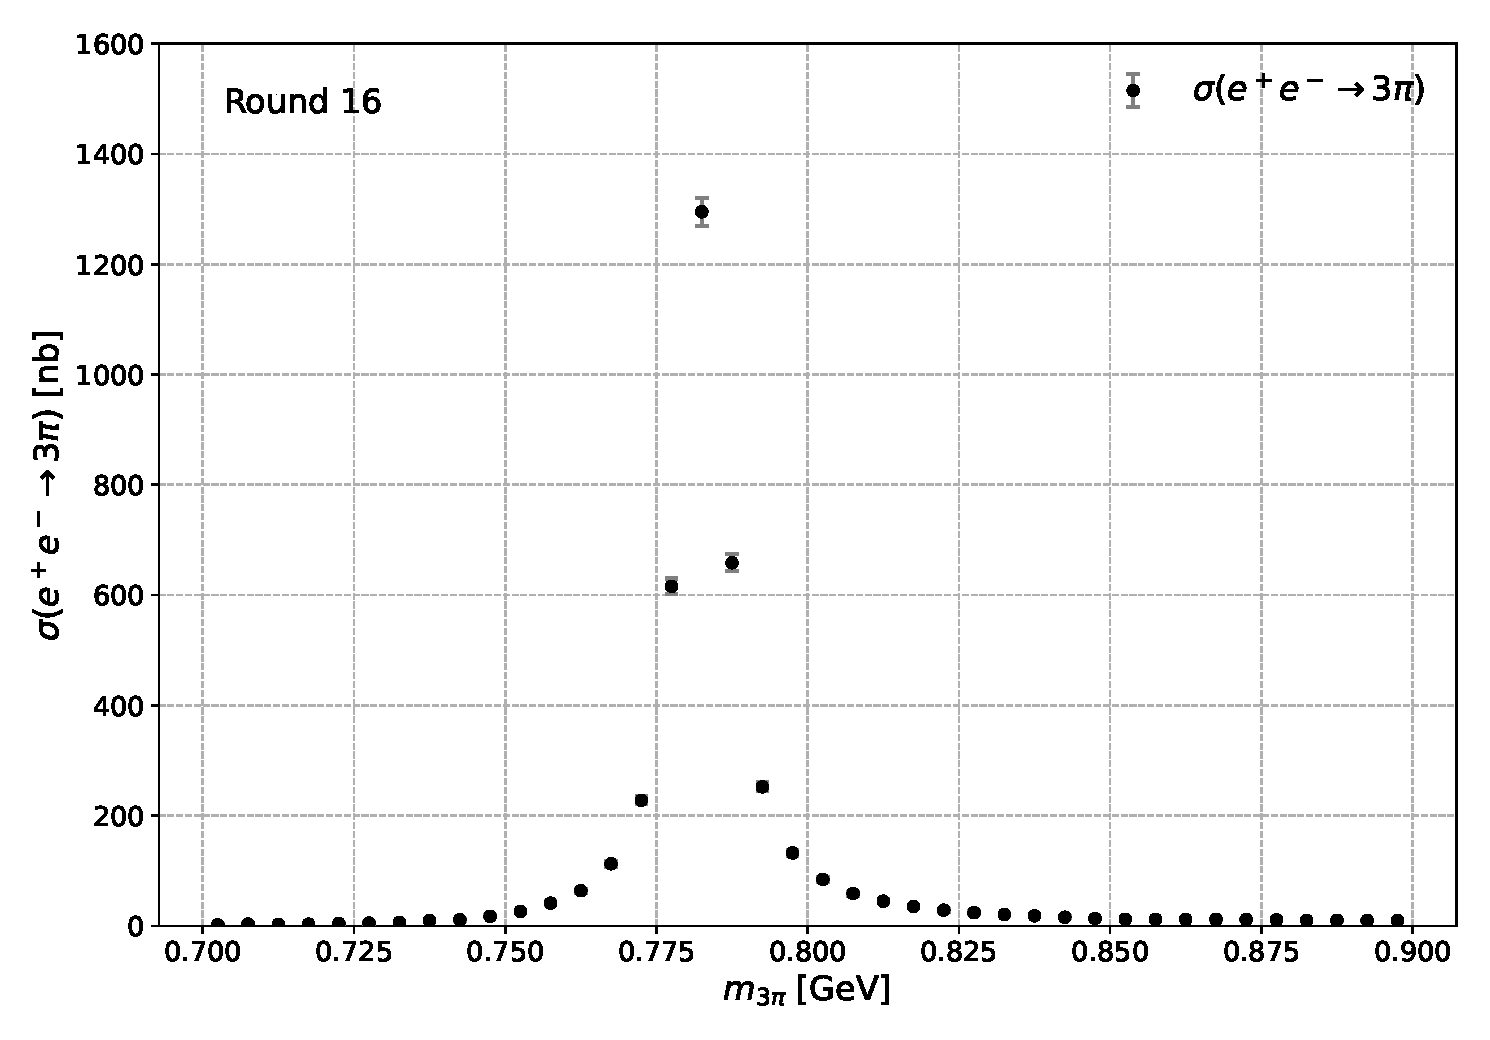
\includegraphics[width=0.32\textwidth]{fig/sigma_final_round16_omega.eps}
        \label{fig:sigma_final_round16_omega}
    }\hfill
    \subfloat[Round 16, $\phi(1020)$ region]{
        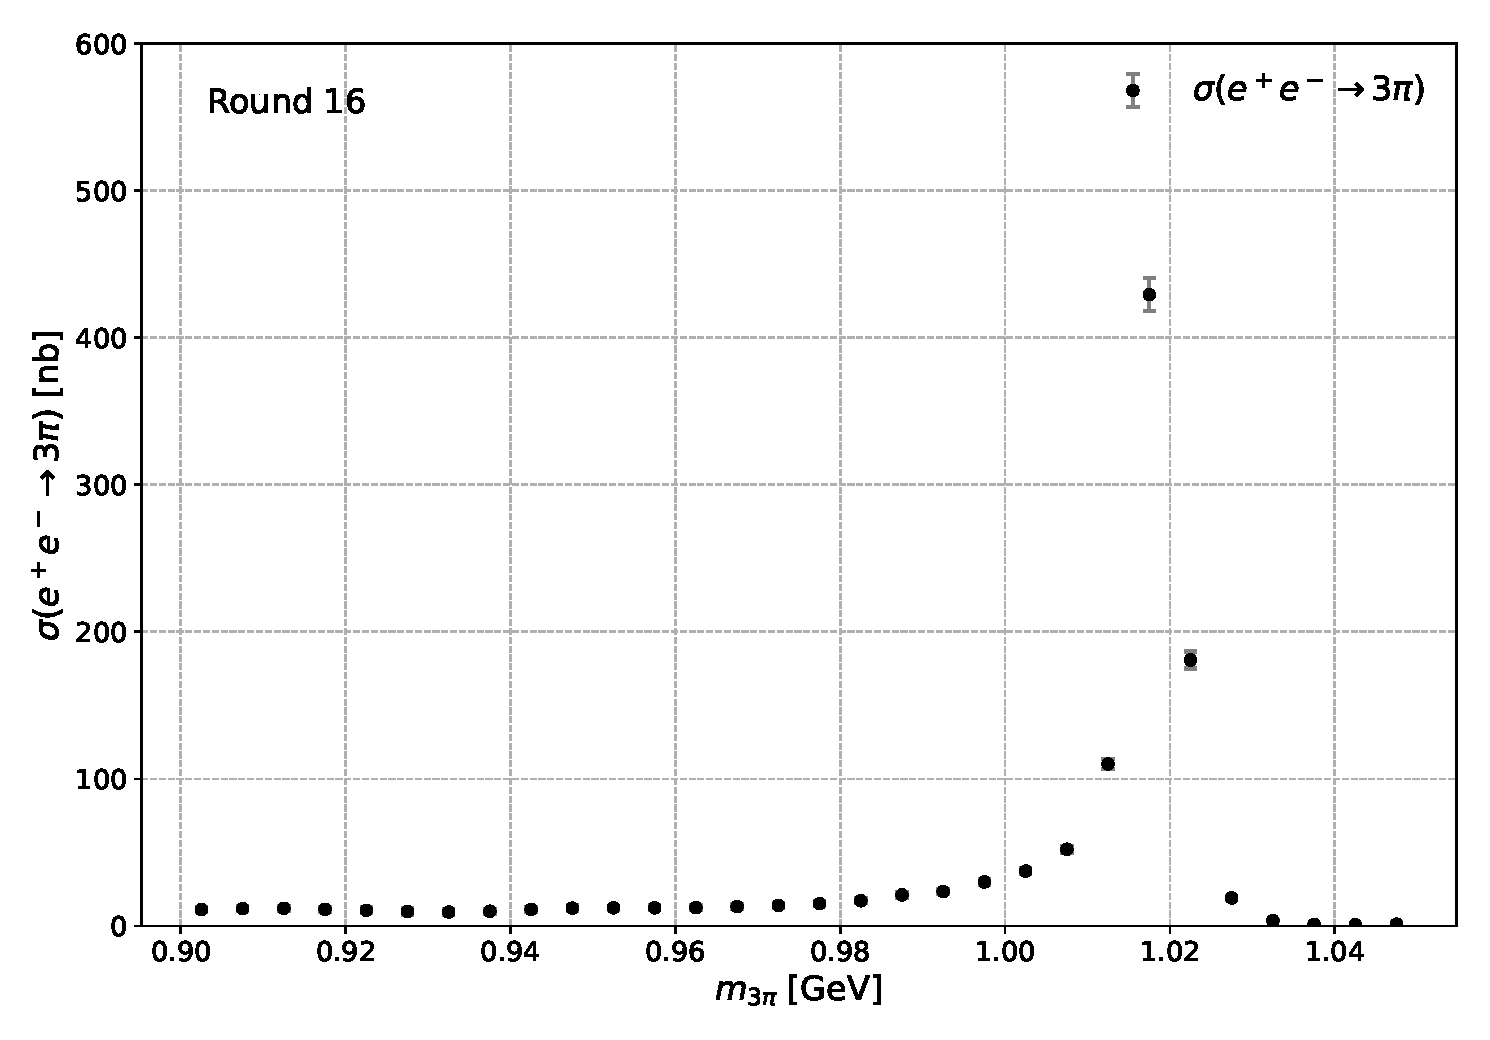
\includegraphics[width=0.32\textwidth]{fig/sigma_final_round16_phi.eps}
        \label{fig:sigma_final_round16_phi}
    }\hfill
    \subfloat[Round 16, $\omega^{\prime}/\omega^{\prime\prime}$ region]{
        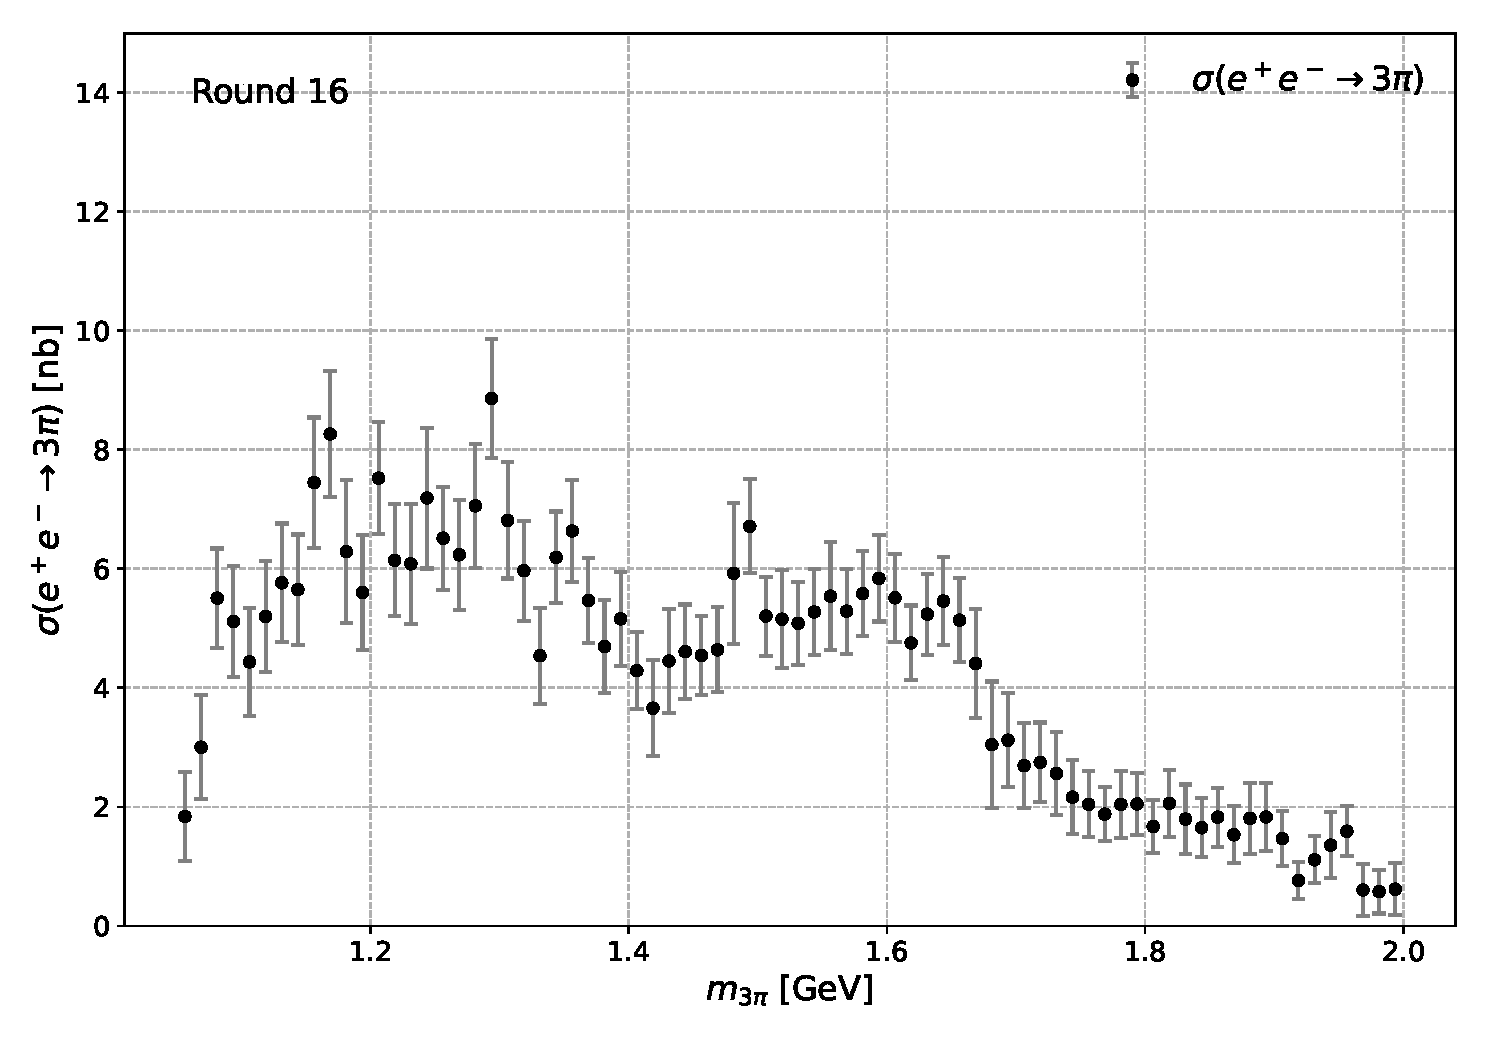
\includegraphics[width=0.32\textwidth]{fig/sigma_final_round16_high.eps}
        \label{fig:sigma_final_round16_high}
    }

    \vspace{0.5\baselineskip}

    % === Row 4: Round 17 ===
    \subfloat[Round 17, $\omega(782)$ region]{
        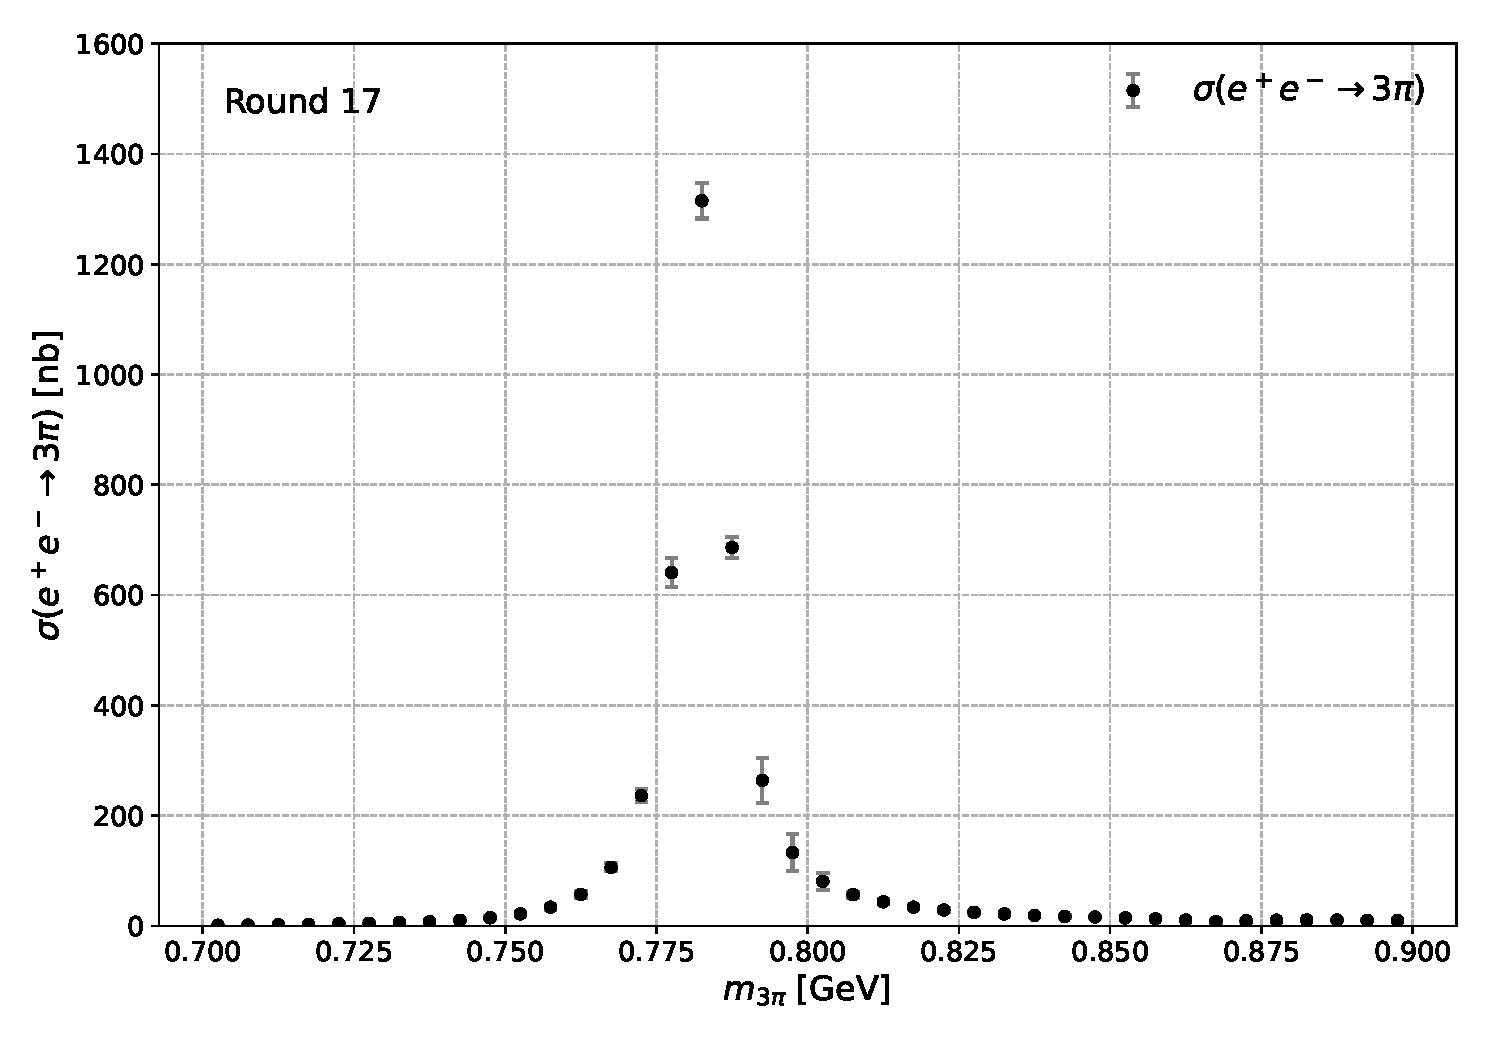
\includegraphics[width=0.32\textwidth]{fig/sigma_final_round17_omega.eps}
        \label{fig:sigma_final_round17_omega}
    }\hfill
    \subfloat[Round 17, $\phi(1020)$ region]{
        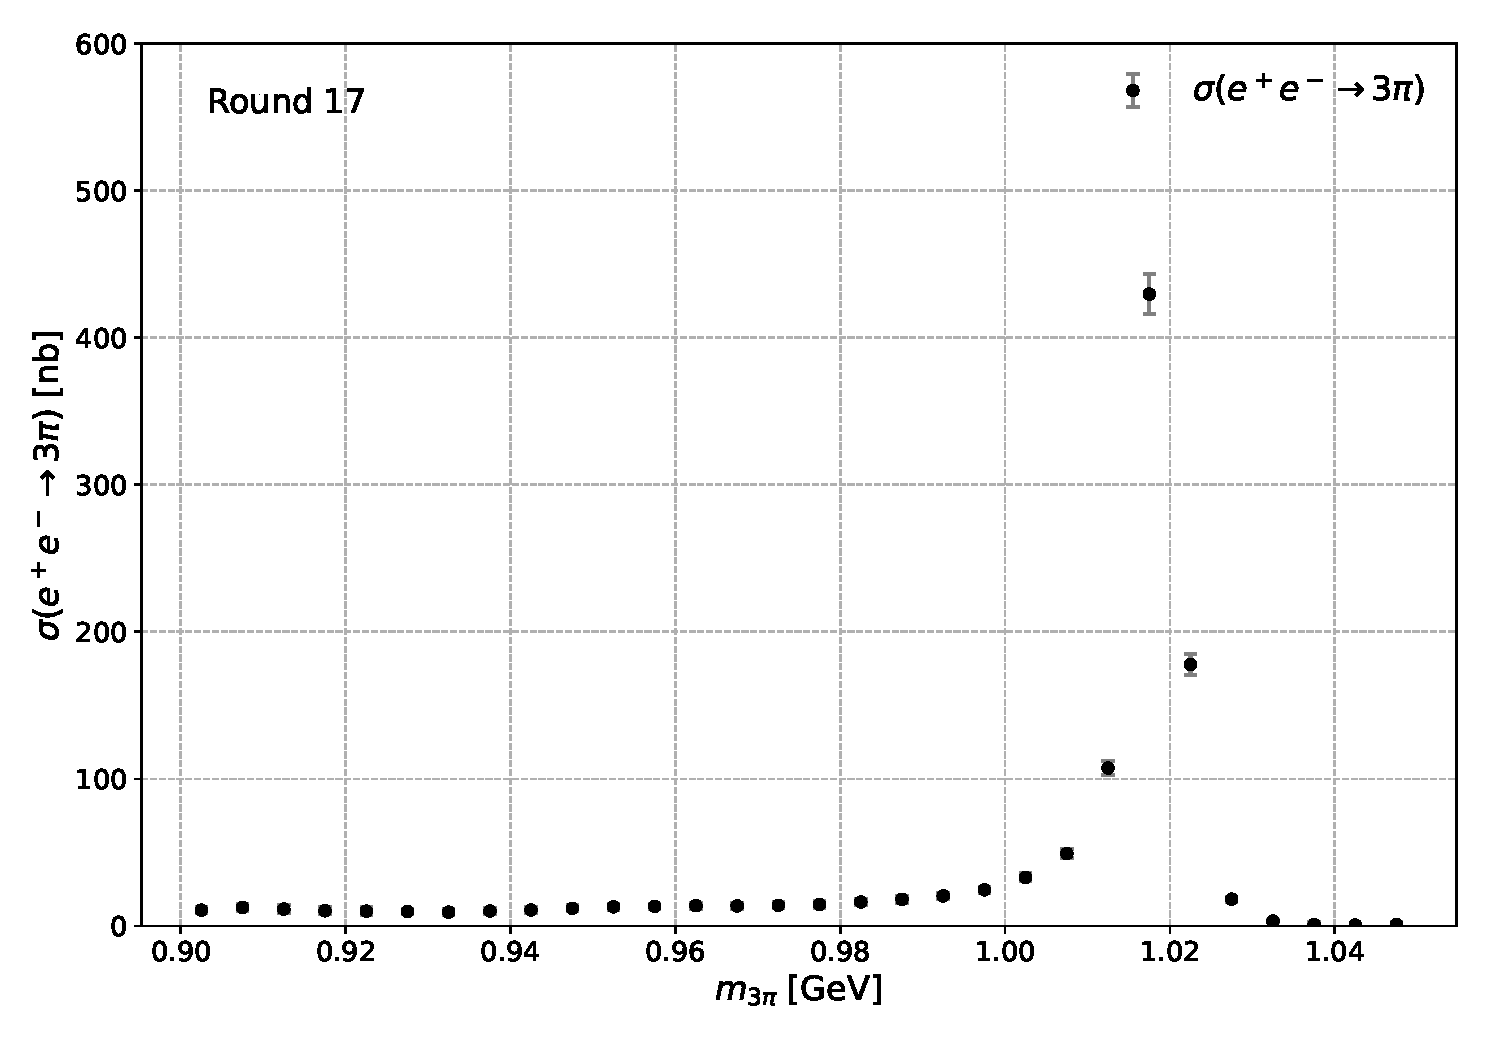
\includegraphics[width=0.32\textwidth]{fig/sigma_final_round17_phi.eps}
        \label{fig:sigma_final_round17_phi}
    }\hfill
    \subfloat[Round 17, $\omega^{\prime}/\omega^{\prime\prime}$ region]{
        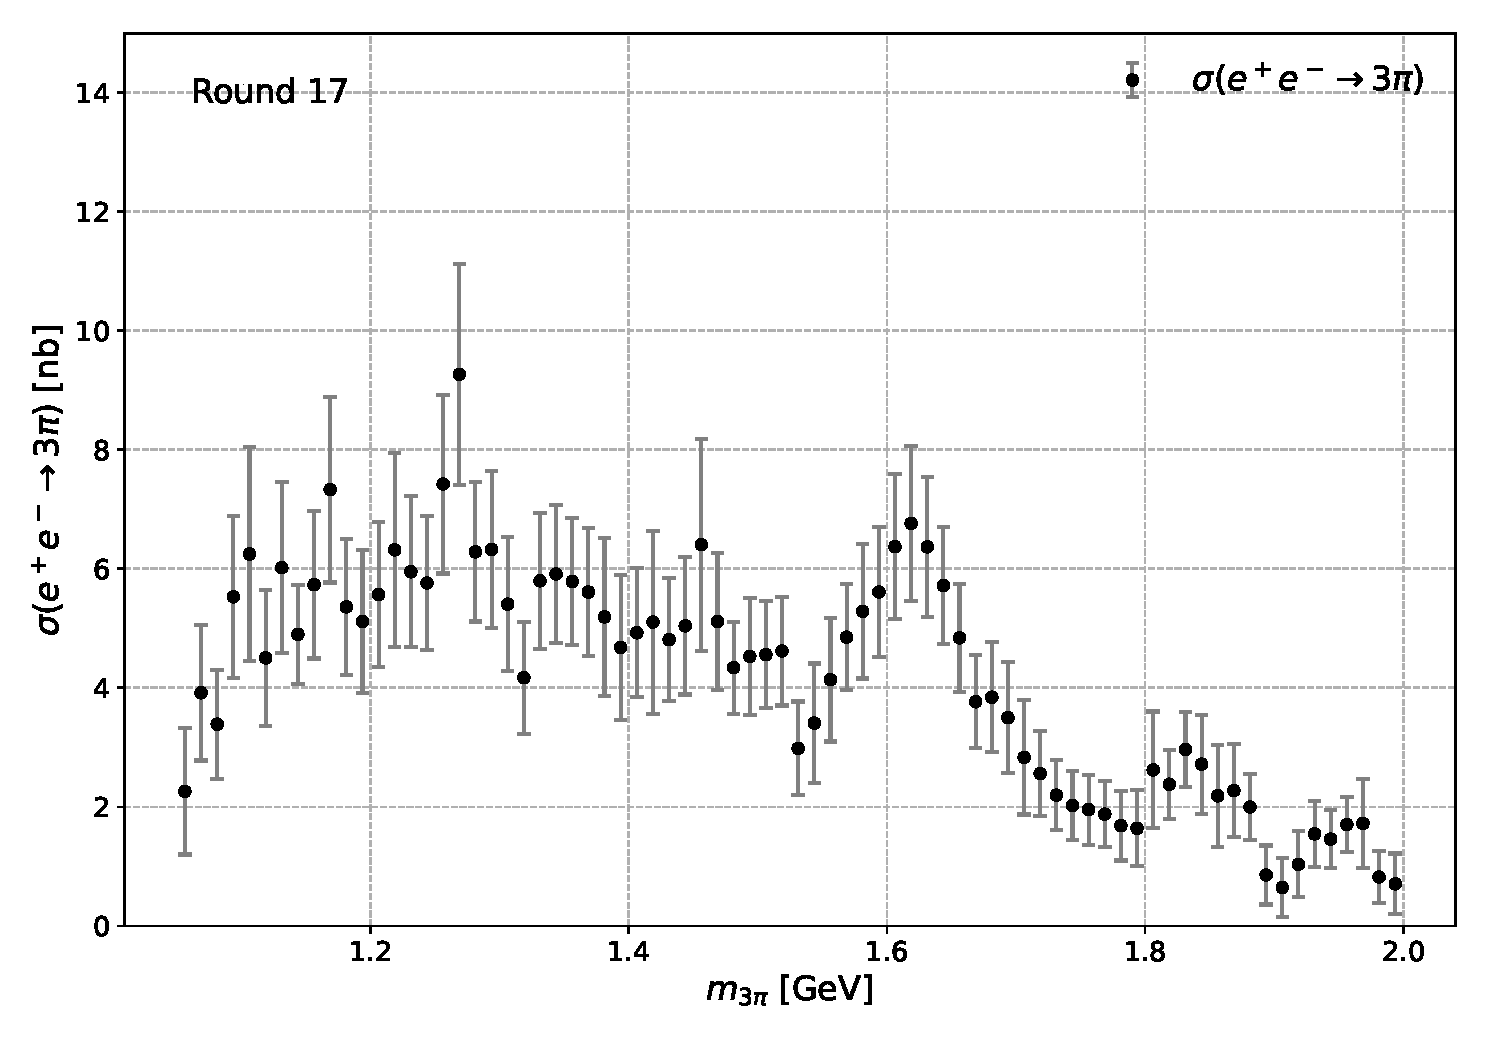
\includegraphics[width=0.32\textwidth]{fig/sigma_final_round17_high.eps}
        \label{fig:sigma_final_round17_high}
    }

    \caption{Dressed cross section $\sigma_{3\pi}^{\text{dress}}(m)$ results for the four independent data-taking periods (Round~03/04, Round~15, Round~16, and Round~17). The uncertainties are derived from the covariance matrices obtained from the unfolding procedure, which fully describe the correlations of the unfolded mass spectrum.}
    \label{fig:sigma_dress_results_all_rounds}
\end{figure}

\clearpage
\subsection{Combination of independent dressed cross section measurements}

Since the four data-taking periods (Round~03/04, Round~15, Round~16, and Round~17) are statistically independent, we can combine their dressed cross section results to obtain a more precise measurement. However, a simple weighted average using only the diagonal uncertainties would be suboptimal, as it neglects the bin-to-bin correlations within each measurement that arise from the unfolding procedure.

To properly account for these correlations, we employ the Best Linear Unbiased Estimator (BLUE) method~\cite{BLUE1,BLUE2}. BLUE provides a systematic framework for combining multiple correlated measurements that estimate the same underlying quantity, producing an estimate that is both unbiased and has minimum variance.

\subsubsection{Formalism of BLUE}

Suppose we have $n$ independent measurements $\mathbf{x}_i$ ($i = 1, \ldots, n$), each being a vector of length $m$ (corresponding to the $m$ invariant mass bins). Each measurement is an unbiased estimator of the true value $\boldsymbol{\mu}$:
\begin{equation}
    E[\mathbf{x}_i] = \boldsymbol{\mu}, \quad \text{Cov}(\mathbf{x}_i) = \mathbf{V}_i
\end{equation}
where $\mathbf{V}_i$ is the $m \times m$ covariance matrix for the $i$-th measurement, which contains both the variances ($\sigma_{i,p}^2$ on the diagonal) and the bin-to-bin covariances ($\rho_{pq}\sigma_{i,p}\sigma_{i,q}$ off-diagonal). Since the measurements are independent, the cross-covariances satisfy $\text{Cov}(\mathbf{x}_i, \mathbf{x}_j) = 0$ for $i \neq j$.

We seek a linear combination of all measurements:
\begin{equation}
    \hat{\boldsymbol{\mu}} = \sum_{i=1}^{n} \mathbf{W}_i \mathbf{x}_i
\end{equation}
where each $\mathbf{W}_i$ is an $m \times m$ weight matrix to be determined. The estimator $\hat{\boldsymbol{\mu}}$ is required to be unbiased:
\begin{equation}
    E[\hat{\boldsymbol{\mu}}] = \sum_{i=1}^{n} \mathbf{W}_i E[\mathbf{x}_i] = \left( \sum_{i=1}^{n} \mathbf{W}_i \right) \boldsymbol{\mu} = \boldsymbol{\mu}
\end{equation}
which imposes the constraint $\sum_{i=1}^{n} \mathbf{W}_i = \mathbf{I}$ (the identity matrix).

The covariance matrix of the combined estimator is:
\begin{equation}
    \mathbf{U} = \text{Cov}(\hat{\boldsymbol{\mu}}) = \sum_{i=1}^{n} \mathbf{W}_i \mathbf{V}_i \mathbf{W}_i^T
\end{equation}
since the cross-terms vanish due to independence.

\subsubsection{Optimal weights}

The BLUE method minimizes the variance (in the sense of matrix trace or any positive-definite metric) subject to the unbiasedness constraint. Solving this optimization problem using Lagrange multipliers yields the optimal weight matrices:
\begin{equation}
    \mathbf{W}_i = \left( \sum_{j=1}^{n} \mathbf{V}_j^{-1} \right)^{-1} \mathbf{V}_i^{-1}
\end{equation}
provided that all $\mathbf{V}_i$ are invertible. If some covariance matrices are singular or near-singular, we use the Moore-Penrose pseudo-inverse instead.

Substituting these weights back gives the combined estimate:
\begin{equation}
    \hat{\boldsymbol{\mu}} = \left( \sum_{i=1}^{n} \mathbf{V}_i^{-1} \right)^{-1} \left( \sum_{i=1}^{n} \mathbf{V}_i^{-1} \mathbf{x}_i \right)
    \label{eq:blue_estimate}
\end{equation}
and its covariance matrix:
\begin{equation}
    \mathbf{U} = \left( \sum_{i=1}^{n} \mathbf{V}_i^{-1} \right)^{-1}
    \label{eq:blue_covariance}
\end{equation}

\subsubsection{Application to this analysis}

We apply the BLUE method to combine the four independent measurements of $\sigma_{3\pi}^{\text{dress}}(m) \cdot \mathcal{B}(\pi^0\to\gamma\gamma)$, each represented by a vector $\mathbf{x}_i$ (size 40 for Region~1, 30 for Region~2, and 76 for Region~3) and its associated covariance matrix $\mathbf{V}_i$ obtained from the unfolding procedure via standard error propagation. The four $\mathbf{V}_i$ are derived from the covariance matrices of the unfolded mass spectra $\left( \frac{dN}{dm} \right)^{\text{gen}}$, scaled by the luminosity factors:
\begin{equation}
    \mathbf{V}_i = \frac{\mathbf{V}_i^{(N)}}{\Delta L_i^2}
\end{equation}
where $\mathbf{V}_i^{(N)}$ is the covariance matrix of the unfolded yield, and $\Delta L_i$ is the integrated luminosity per mass bin for the $i$-th period. Note that the branching fraction $\mathcal{B}(\pi^0\to\gamma\gamma)$ is intentionally omitted here, as it will be applied after the combination to allow for separate treatment of its systematic uncertainty.

The combined result $\hat{\boldsymbol{\mu}}_{\text{withBR}}$ therefore represents the best estimate of $\sigma_{3\pi}^{\text{dress}}(m) \cdot \mathcal{B}(\pi^0\to\gamma\gamma)$, with its covariance matrix $\mathbf{U}$ given by Eq.~(\ref{eq:blue_covariance}). The final dressed cross section is obtained by dividing by the central value of the branching fraction:
\begin{equation}
    \hat{\boldsymbol{\mu}}_{\text{dressed}} = \frac{\hat{\boldsymbol{\mu}}_{\text{withBR}}}{\mathcal{B}(\pi^0\to\gamma\gamma)}, \qquad
    \mathbf{U}_{\text{dressed}} = \frac{\mathbf{U}}{\mathcal{B}(\pi^0\to\gamma\gamma)^2}
\end{equation}
The covariance matrix $\mathbf{U}_{\text{dressed}}$ accounts for all statistical uncertainties propagated from the unfolding procedure. The systematic uncertainty due to the branching fraction is not included here and will be treated separately in Sec.~\ref{sec:sys_uncertainties}, as the final dressed cross section is not the ultimate physical quantity of interest in this analysis.

Figure~\ref{fig:blue_merged_results} shows the BLUE-combined dressed cross section results for the three invariant mass regions: the $\omega(782)$ region ($0.7-0.9$~GeV), the $\phi(1020)$ region ($0.9-1.05$~GeV), and the $\omega^{\prime}/\omega^{\prime\prime}$ region ($1.05-2.0$~GeV). The combined result exhibits significantly improved precision compared to individual measurements, particularly in the $\omega(782)$ region where the statistical uncertainties dominate.

\begin{figure}[htbp]
    \centering
    
    \subfloat[$\omega(782)$ region]{
        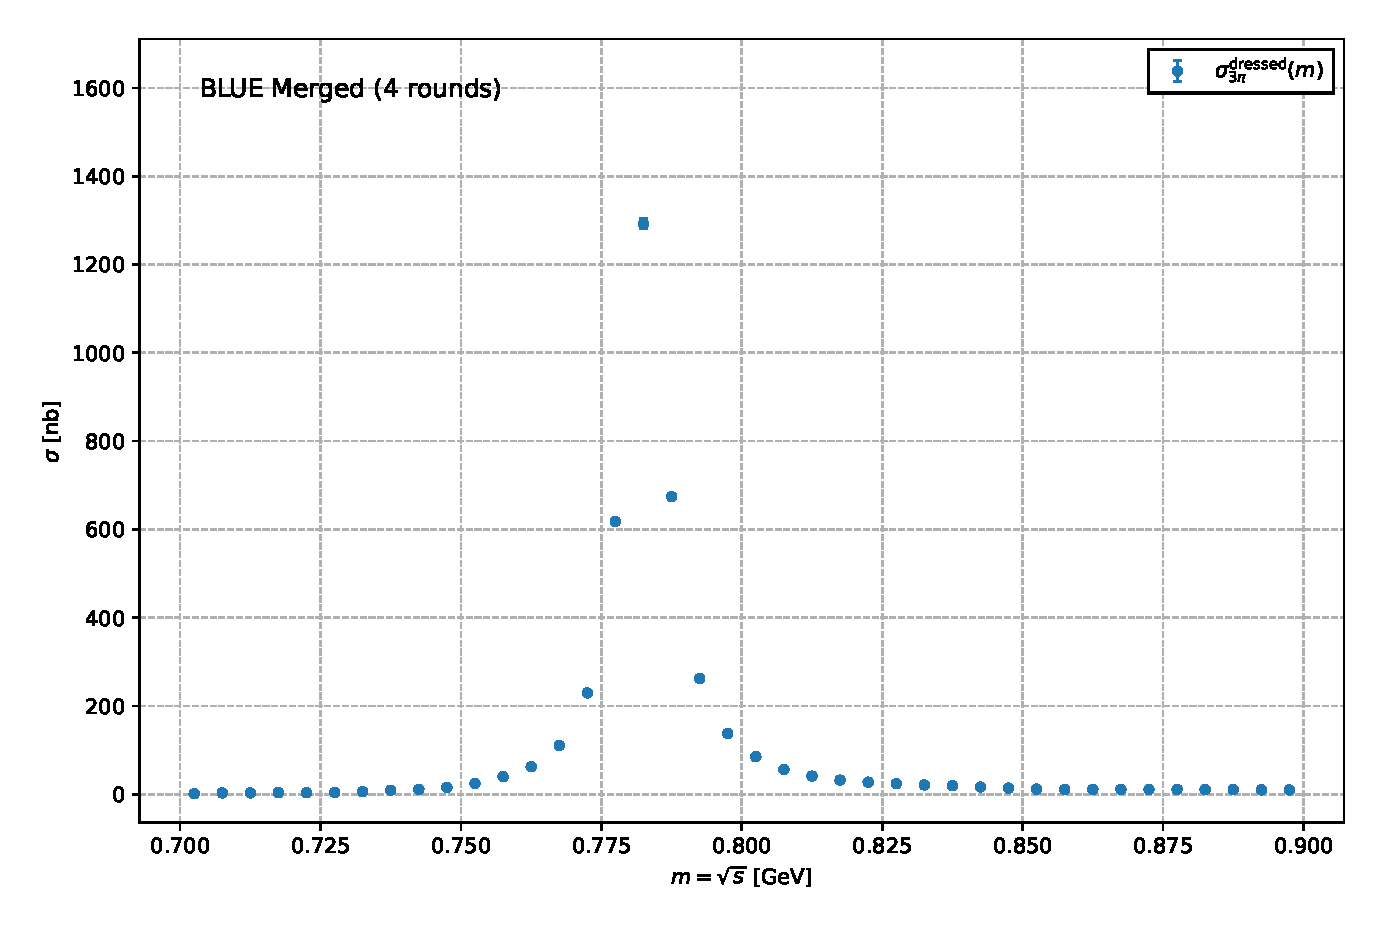
\includegraphics[width=0.32\textwidth]{fig/blue_merged_region1.eps}
        \label{fig:blue_merged_region1}
    }\hfill
    \subfloat[$\phi(1020)$ region]{
        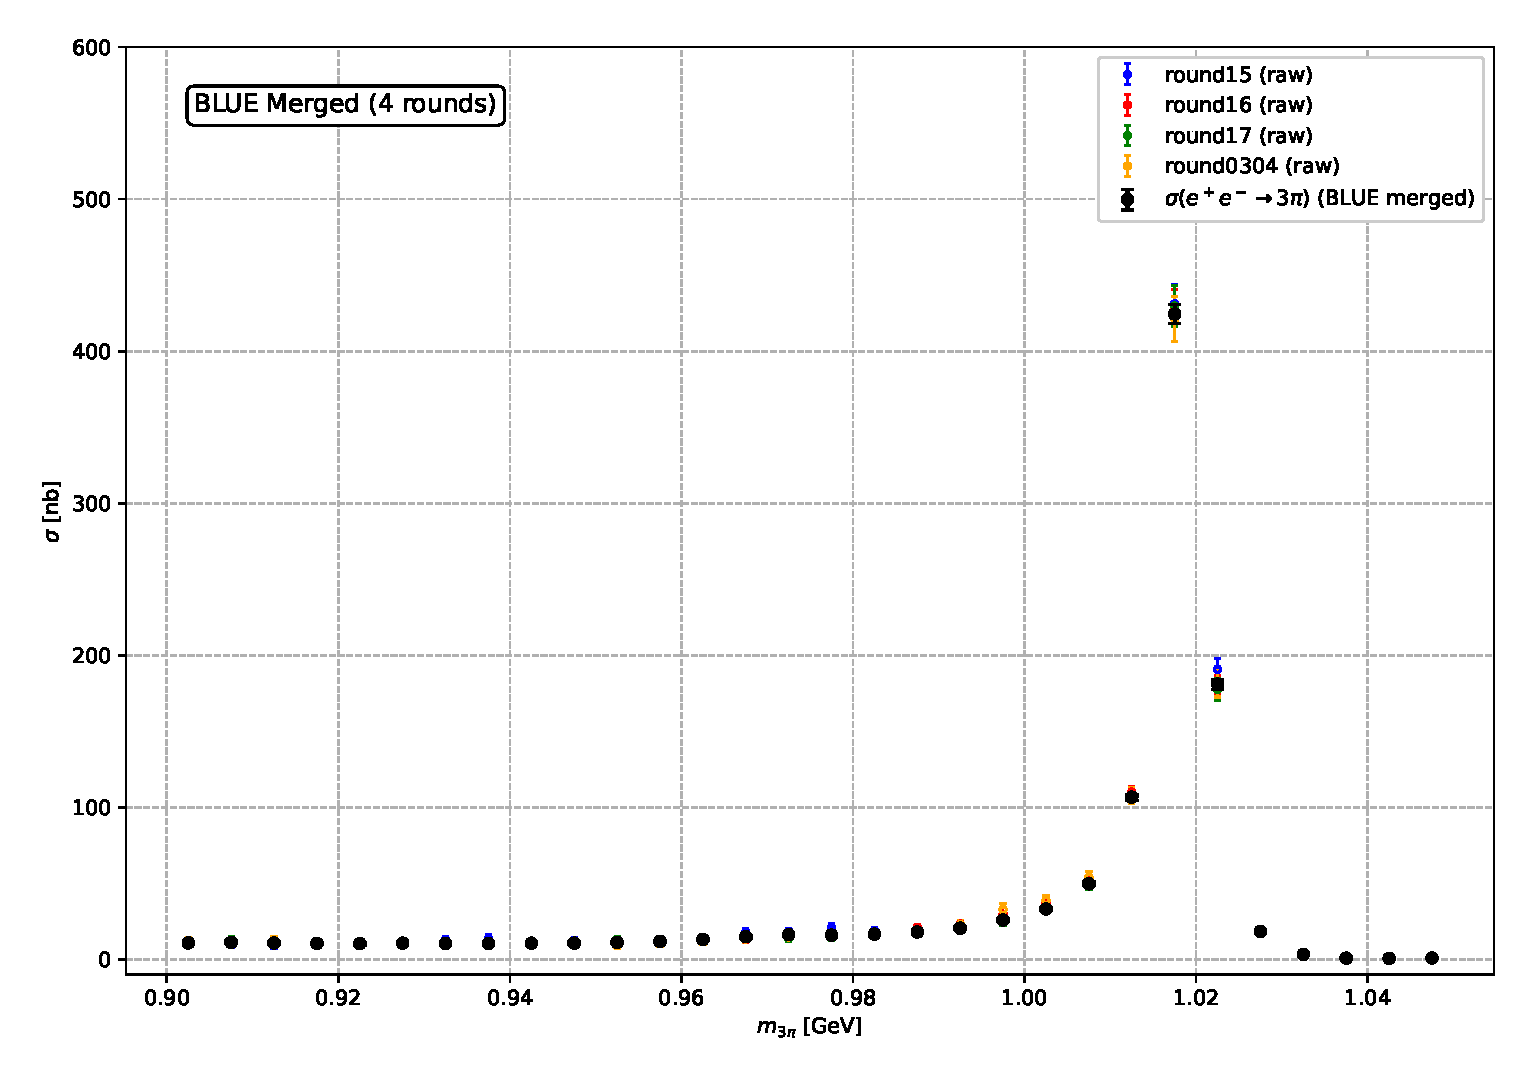
\includegraphics[width=0.32\textwidth]{fig/blue_merged_region2.eps}
        \label{fig:blue_merged_region2}
    }\hfill
    \subfloat[$\omega^{\prime}/\omega^{\prime\prime}$ region]{
        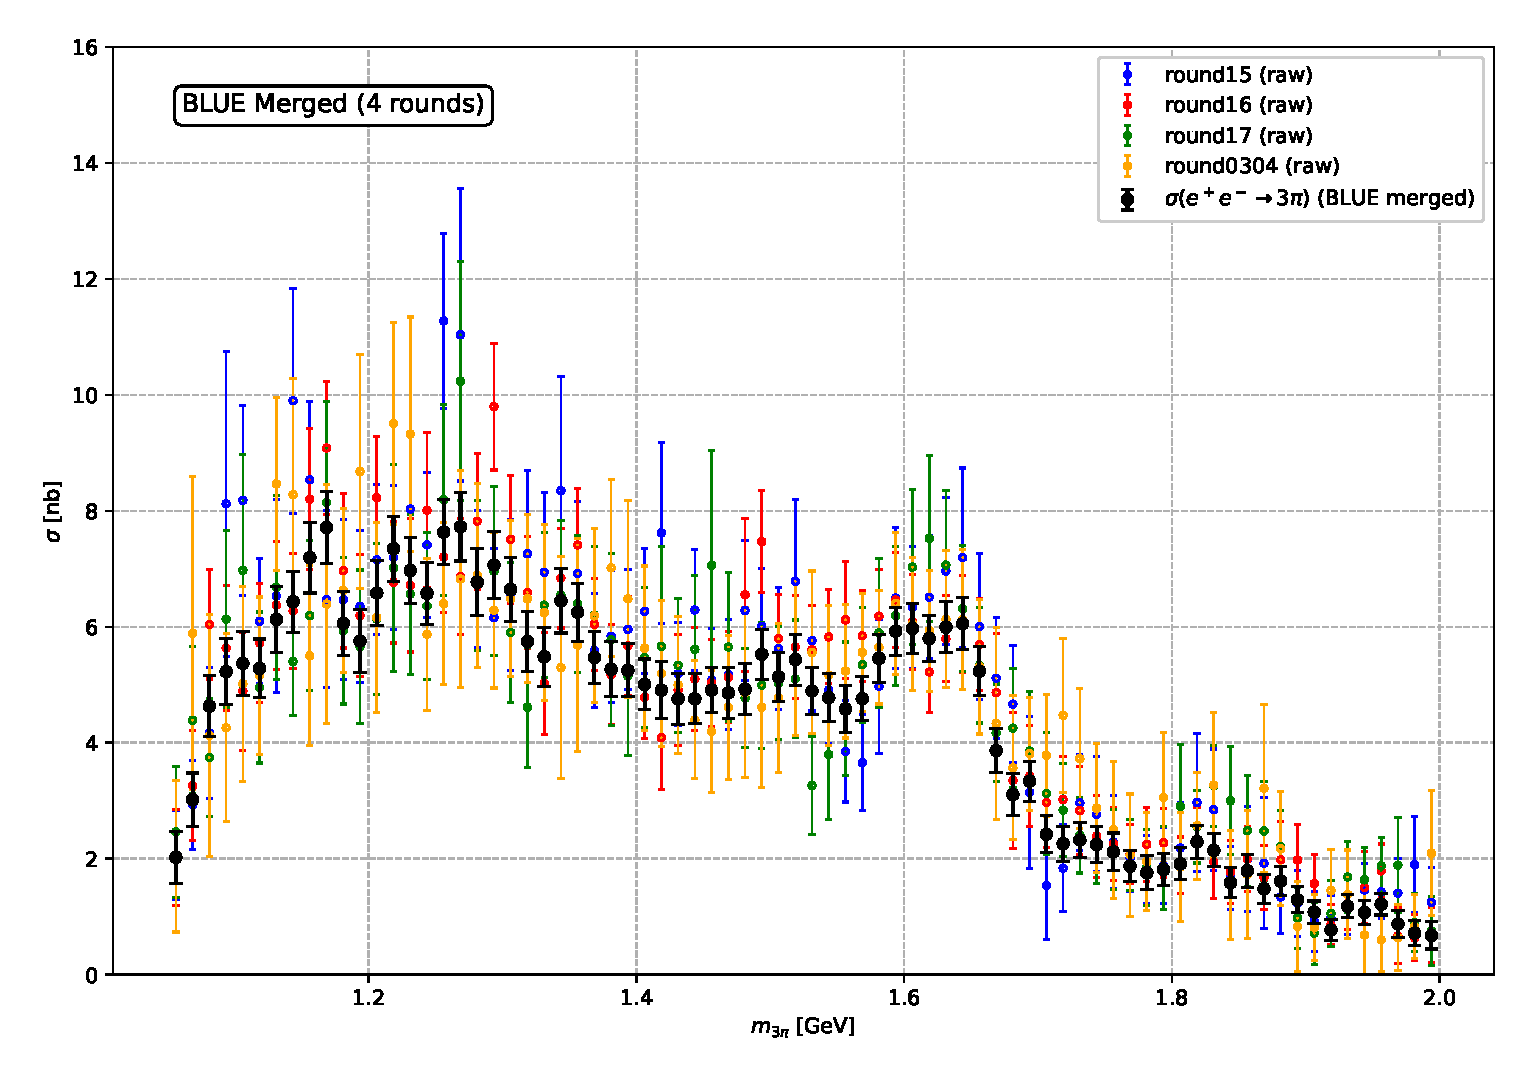
\includegraphics[width=0.32\textwidth]{fig/blue_merged_region3.eps}
        \label{fig:blue_merged_region3}
    }
    
    \caption{BLUE-combined dressed cross section $\sigma_{3\pi}^{\text{dress}}(m)$ results for the three invariant mass regions. The error bars represent the statistical uncertainties propagated from the covariance matrices. The combination significantly improves the statistical precision compared to any single data-taking period.}
    \label{fig:blue_merged_results}
\end{figure}

For completeness, Fig.~\ref{fig:blue_merged_all_regions} presents the combined results across all three regions on a logarithmic scale, illustrating the full spectrum from $0.7$ to $2.0$~GeV in a single view.

\begin{figure}[htbp]
    \centering
    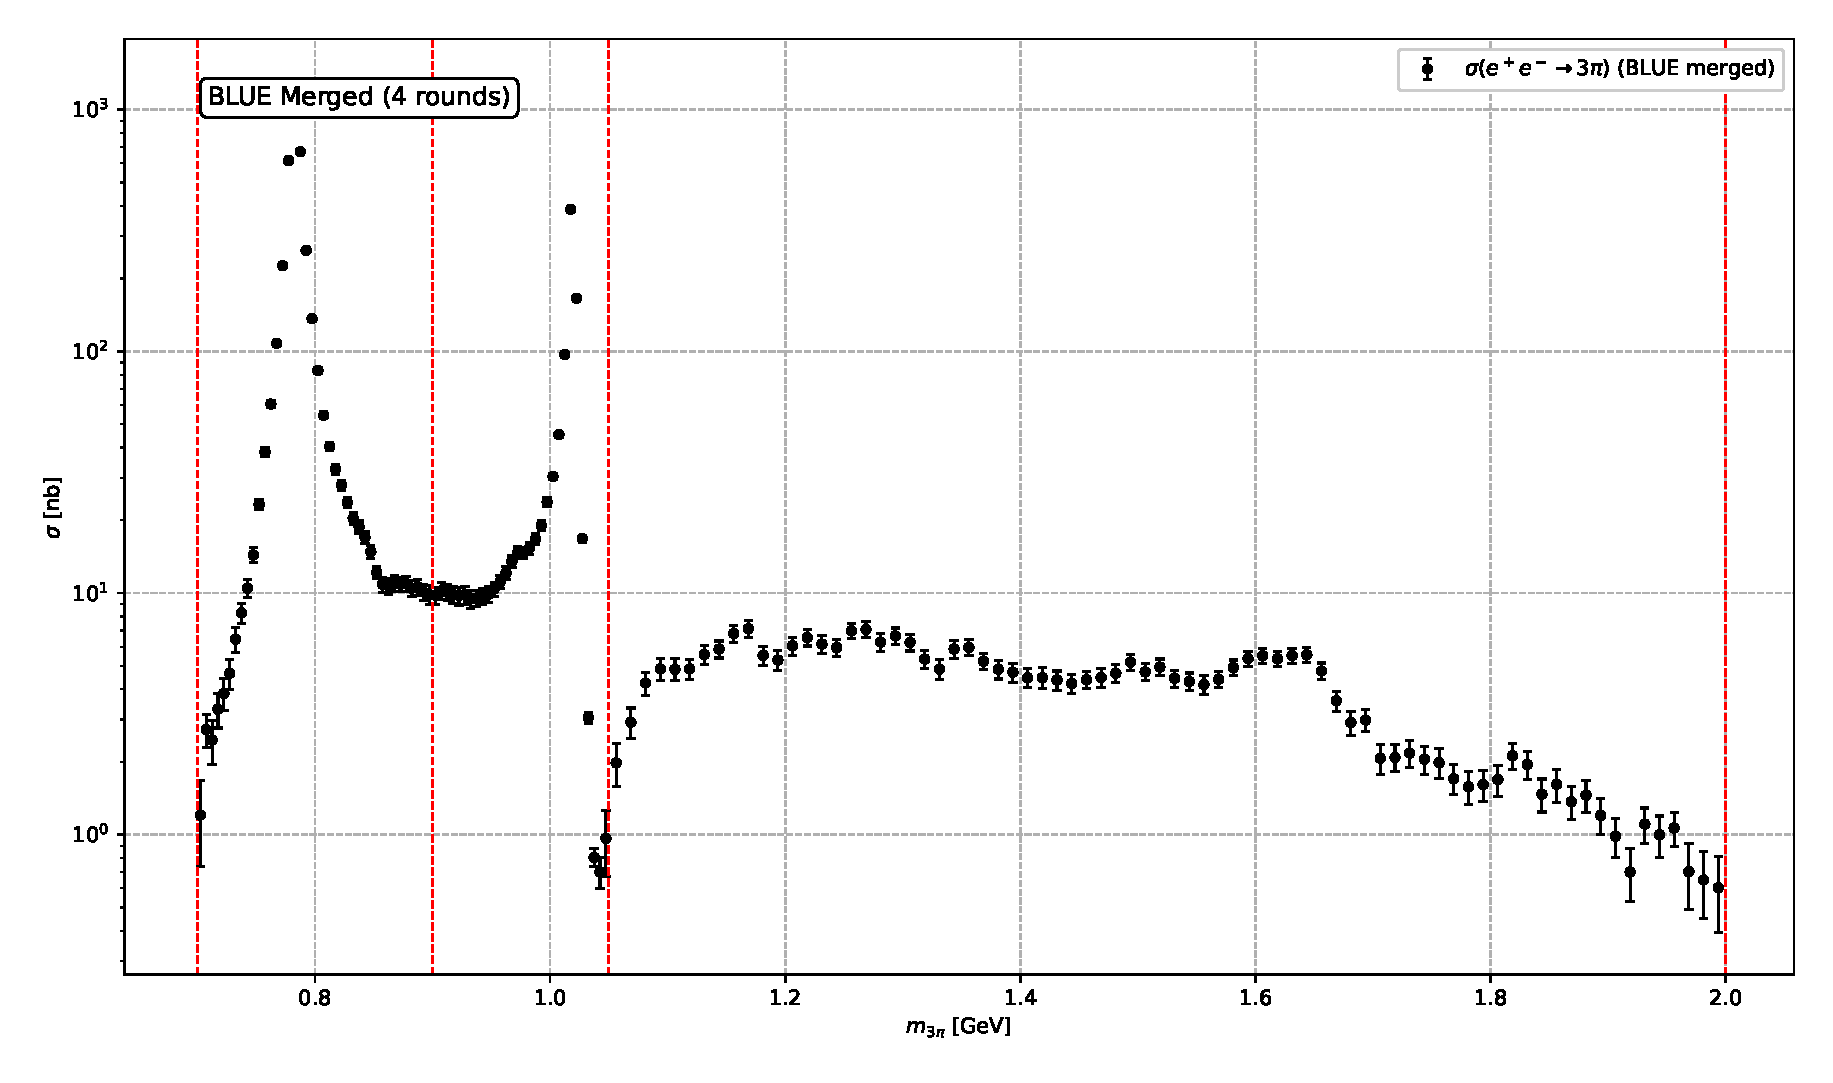
\includegraphics[width=0.75\textwidth]{fig/blue_merged_all_regions.eps}
    \caption{BLUE-combined dressed cross section $\sigma_{3\pi}^{\text{dress}}(m)$ across all three invariant mass regions, shown on a logarithmic scale.}
    \label{fig:blue_merged_all_regions}
\end{figure}